\documentclass[12pt]{beamer}\usepackage[]{graphicx}\usepackage[]{color}
%% maxwidth is the original width if it is less than linewidth
%% otherwise use linewidth (to make sure the graphics do not exceed the margin)
\makeatletter
\def\maxwidth{ %
  \ifdim\Gin@nat@width>\linewidth
    \linewidth
  \else
    \Gin@nat@width
  \fi
}
\makeatother

\definecolor{fgcolor}{rgb}{0.345, 0.345, 0.345}
\newcommand{\hlnum}[1]{\textcolor[rgb]{0.686,0.059,0.569}{#1}}%
\newcommand{\hlstr}[1]{\textcolor[rgb]{0.192,0.494,0.8}{#1}}%
\newcommand{\hlcom}[1]{\textcolor[rgb]{0.678,0.584,0.686}{\textit{#1}}}%
\newcommand{\hlopt}[1]{\textcolor[rgb]{0,0,0}{#1}}%
\newcommand{\hlstd}[1]{\textcolor[rgb]{0.345,0.345,0.345}{#1}}%
\newcommand{\hlkwa}[1]{\textcolor[rgb]{0.161,0.373,0.58}{\textbf{#1}}}%
\newcommand{\hlkwb}[1]{\textcolor[rgb]{0.69,0.353,0.396}{#1}}%
\newcommand{\hlkwc}[1]{\textcolor[rgb]{0.333,0.667,0.333}{#1}}%
\newcommand{\hlkwd}[1]{\textcolor[rgb]{0.737,0.353,0.396}{\textbf{#1}}}%

\usepackage{framed}
\makeatletter
\newenvironment{kframe}{%
 \def\at@end@of@kframe{}%
 \ifinner\ifhmode%
  \def\at@end@of@kframe{\end{minipage}}%
  \begin{minipage}{\columnwidth}%
 \fi\fi%
 \def\FrameCommand##1{\hskip\@totalleftmargin \hskip-\fboxsep
 \colorbox{shadecolor}{##1}\hskip-\fboxsep
     % There is no \\@totalrightmargin, so:
     \hskip-\linewidth \hskip-\@totalleftmargin \hskip\columnwidth}%
 \MakeFramed {\advance\hsize-\width
   \@totalleftmargin\z@ \linewidth\hsize
   \@setminipage}}%
 {\par\unskip\endMakeFramed%
 \at@end@of@kframe}
\makeatother

\definecolor{shadecolor}{rgb}{.97, .97, .97}
\definecolor{messagecolor}{rgb}{0, 0, 0}
\definecolor{warningcolor}{rgb}{1, 0, 1}
\definecolor{errorcolor}{rgb}{1, 0, 0}
\newenvironment{knitrout}{}{} % an empty environment to be redefined in TeX

\usepackage{alltt}
\usepackage{graphicx}
\usepackage{tikz}
\setbeameroption{hide notes}
\setbeamertemplate{note page}[plain]
\usepackage{listings}

% get rid of junk
\usetheme{default}
\usefonttheme[onlymath]{serif}
\beamertemplatenavigationsymbolsempty
\hypersetup{pdfpagemode=UseNone} % don't show bookmarks on initial view

% named colors
\definecolor{offwhite}{RGB}{255,250,240}
\definecolor{gray}{RGB}{155,155,155}

\ifx\notescolors\undefined % slides

  \definecolor{foreground}{RGB}{80,80,80}
  \definecolor{background}{RGB}{255,255,255}
  \definecolor{title}{RGB}{255,199,0}
  \definecolor{subtitle}{RGB}{89,132,212}
  \definecolor{hilit}{RGB}{248,117,79}
  \definecolor{vhilit}{RGB}{255,111,207}
  \definecolor{lolit}{RGB}{200,200,200}
  \definecolor{lit}{RGB}{255,199,0}
  \definecolor{mdlit}{RGB}{89,132,212}
  \definecolor{link}{RGB}{248,117,79}

\else % notes
  \definecolor{background}{RGB}{255,255,255}
  \definecolor{foreground}{RGB}{24,24,24}
  \definecolor{title}{RGB}{27,94,134}
  \definecolor{subtitle}{RGB}{22,175,124}
  \definecolor{hilit}{RGB}{122,0,128}
  \definecolor{vhilit}{RGB}{255,0,128}
  \definecolor{lolit}{RGB}{95,95,95}
\fi
\definecolor{nhilit}{RGB}{128,0,128}  % hilit color in notes
\definecolor{nvhilit}{RGB}{255,0,128} % vhilit for notes

\newcommand{\hilit}{\color{hilit}}
\newcommand{\vhilit}{\color{vhilit}}
\newcommand{\nhilit}{\color{nhilit}}
\newcommand{\nvhilit}{\color{nvhilit}}
\newcommand{\lit}{\color{lit}}
\newcommand{\mdlit}{\color{mdlit}}
\newcommand{\lolit}{\color{lolit}}

% use those colors
\setbeamercolor{titlelike}{fg=title}
\setbeamercolor{subtitle}{fg=subtitle}
\setbeamercolor{frametitle}{fg=gray}
\setbeamercolor{structure}{fg=subtitle}
\setbeamercolor{institute}{fg=lolit}
\setbeamercolor{normal text}{fg=foreground,bg=background}
%\setbeamercolor{item}{fg=foreground} % color of bullets
%\setbeamercolor{subitem}{fg=hilit}
%\setbeamercolor{itemize/enumerate subbody}{fg=lolit}
\setbeamertemplate{itemize subitem}{{\textendash}}
\setbeamerfont{itemize/enumerate subbody}{size=\footnotesize}
\setbeamerfont{itemize/enumerate subitem}{size=\footnotesize}

% center title of slides
\setbeamertemplate{blocks}[rounded]
\setbeamertemplate{frametitle}[default][center]
% margins
\setbeamersize{text margin left=25pt,text margin right=25pt}

% page number
\setbeamertemplate{footline}{%
    \raisebox{5pt}{\makebox[\paperwidth]{\hfill\makebox[20pt]{\lolit
          \scriptsize\insertframenumber}}}\hspace*{5pt}}

% add a bit of space at the top of the notes page
\addtobeamertemplate{note page}{\setlength{\parskip}{12pt}}

% default link color
\hypersetup{colorlinks, urlcolor={link}}

\ifx\notescolors\undefined % slides
  % set up listing environment
  \lstset{language=bash,
          basicstyle=\ttfamily\scriptsize,
          frame=single,
          commentstyle=,
          backgroundcolor=\color{darkgray},
          showspaces=false,
          showstringspaces=false
          }
\else % notes
  \lstset{language=bash,
          basicstyle=\ttfamily\scriptsize,
          frame=single,
          commentstyle=,
          backgroundcolor=\color{offwhite},
          showspaces=false,
          showstringspaces=false
          }
\fi

% a few macros
\newcommand{\code}[1]{\texttt{#1}}
\newcommand{\hicode}[1]{{\hilit \texttt{#1}}}
\newcommand{\bb}[1]{\begin{block}{#1}}
\newcommand{\eb}{\end{block}}
\newcommand{\bi}{\begin{itemize}}
%\newcommand{\bbi}{\vspace{24pt} \begin{itemize} \itemsep8pt}
\newcommand{\bbi}{\vspace{4pt} \begin{itemize} \itemsep8pt}
\newcommand{\ei}{\end{itemize}}
\newcommand{\bv}{\begin{verbatim}}
\newcommand{\ev}{\end{verbatim}}
\newcommand{\ig}{\includegraphics}
\newcommand{\subt}[1]{{\footnotesize \color{subtitle} {#1}}}
\newcommand{\ttsm}{\tt \small}
\newcommand{\ttfn}{\tt \footnotesize}
\newcommand{\figh}[2]{\centerline{\includegraphics[height=#2\textheight]{#1}}}
\newcommand{\figw}[2]{\centerline{\includegraphics[width=#2\textwidth]{#1}}}



%------------------------------------------------
% end of header
%------------------------------------------------

\title{Univariate Graphics}
\subtitle{STAT 133}
\author{\href{http://www.gastonsanchez.com}{Gaston Sanchez}}
\institute{Department of Statistics, UC{\textendash}Berkeley}
\date{\href{http://www.gastonsanchez.com}{\tt \scriptsize \color{foreground} gastonsanchez.com}
\\[-4pt]
\href{http://github.com/gastonstat/stat133}{\tt \scriptsize \color{foreground} github.com/gastonstat/stat133}
\\[-4pt]
{\scriptsize Course web: \href{http://www.gastonsanchez.com/stat133}{\tt gastonsanchez.com/stat133}}
}
\IfFileExists{upquote.sty}{\usepackage{upquote}}{}
\begin{document}


{
  \setbeamertemplate{footline}{} % no page number here
  \frame{
    \titlepage
  } 
}

%------------------------------------------------

\begin{frame}
\begin{center}
\Huge{\hilit{Looking at one single variable}}
\end{center}
\end{frame}

%------------------------------------------------

\begin{frame}
\frametitle{Univariate Statistical Graphics}
\begin{center}
\large{Getting started with graphics for exploration requires underdstanding charts and plots for single variables}
\pause

\bigskip
\large{Many multivariate graphics are extensions or combinations of univariate charts}

\end{center}
\end{frame}

%------------------------------------------------

\begin{frame}[fragile]
\frametitle{Univariate graphics by type of variable}

\begin{columns}[t]
\begin{column}{0.4\textwidth}
Qualitative Variable
\bi
  \item Bar chart
  \item Dot chart
  \item Pie chart
  \item Pareto chart
\ei
\end{column}

\begin{column}{0.5\textwidth}
Quantitative Variable
\bi
  \item All of qualitative
  \item Histogram
  \item Density curve
  \item Boxplot
  \item Ogive
\ei
\end{column}
\end{columns}

\end{frame}

%------------------------------------------------

\begin{frame}
\begin{center}
\Huge{\hilit{Bar Charts}}
\end{center}
\end{frame}

%------------------------------------------------

\begin{frame}
\frametitle{From Frequency Tables ...}

{\large
\begin{center}
 \begin{tabular}{c c c}
  \hline
  Category & Absolute & Relative \\
   & Frequency & Frequency \\
  \hline
  $C_1$ & $f_1$ & $f_1 / n$ \\
  $C_2$ & $f_2$ & $f_2 / n$ \\
  $C_3$ & $f_3$ & $f_3 / n$ \\
  $\dots$ & $\dots$ & $\dots$ \\
  $C_k$ & $f_k$ & $f_k / n$ \\
  \hline
  $total$ & $n$ & $1$ \\
 \end{tabular}
\end{center}
}

\end{frame}

%------------------------------------------------

\begin{frame}
\frametitle{to Bar-charts}

\begin{knitrout}\footnotesize
\definecolor{shadecolor}{rgb}{0.969, 0.969, 0.969}\color{fgcolor}

{\centering 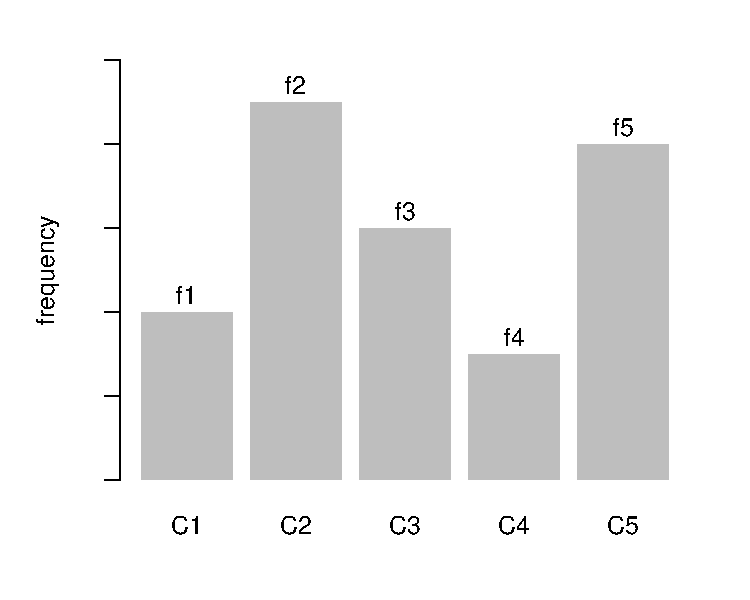
\includegraphics[width=.7\linewidth,height=.6\linewidth]{figure/unnamed-chunk-1-1} 

}



\end{knitrout}

\end{frame}

%------------------------------------------------

\begin{frame}
\frametitle{Bar-charts}

\bb{Elements of vertical bar-charts}
\bi
  \item categories on horizontal axis
  \item frequencies on vertical axis
  \item length of bar equal to frequency
\ei
\eb

(Note that you can also make a horizontal bar-chart, in which case the axes play inverse roles)
\end{frame}

%------------------------------------------------

\begin{frame}
\frametitle{Bar-chart: predominant color in flags}
\begin{center}
\ig[width=9cm]{images/flags.pdf}
\end{center}
\end{frame}

%------------------------------------------------

\begin{frame}[fragile]
\frametitle{Predominant Color in Flags}



\begin{knitrout}\footnotesize
\definecolor{shadecolor}{rgb}{0.969, 0.969, 0.969}\color{fgcolor}\begin{kframe}
\begin{verbatim}
##     color  count  percent
## 1   black      5     2.58
## 2    blue     40    20.62
## 3   brown      2     1.03
## 4    gold     19     9.79
## 5   green     31    15.98
## 6  orange      4     2.06
## 7     red     71    36.60
## 8   white     22    11.34
\end{verbatim}
\end{kframe}
\end{knitrout}

\end{frame}

%------------------------------------------------

\begin{frame}[fragile]
\frametitle{Bar-chart example}

\begin{knitrout}\footnotesize
\definecolor{shadecolor}{rgb}{0.969, 0.969, 0.969}\color{fgcolor}

{\centering 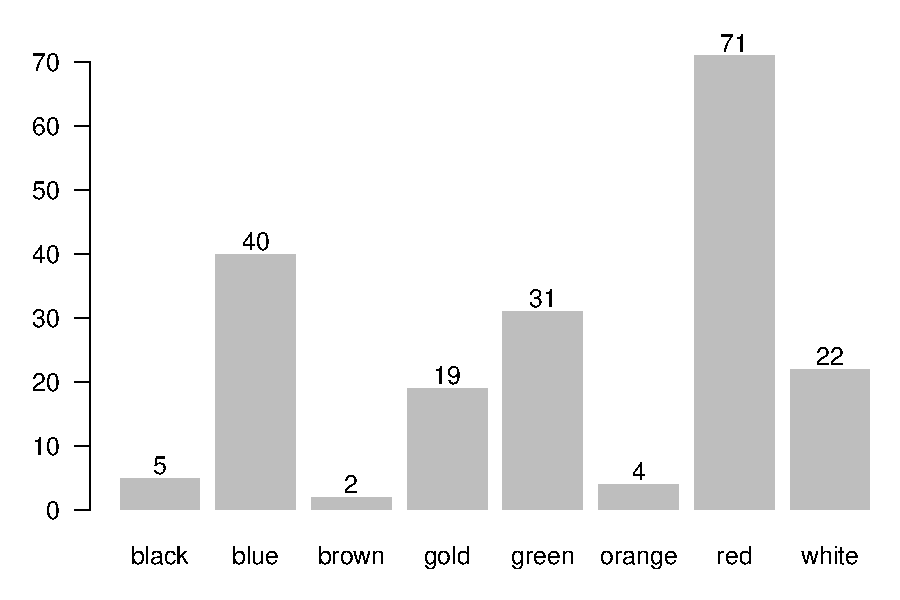
\includegraphics[width=.8\linewidth,height=.6\linewidth]{figure/unnamed-chunk-4-1} 

}



\end{knitrout}

\end{frame}

%------------------------------------------------

\begin{frame}[fragile]
\frametitle{Bar-chart: predominant color in flags}

\begin{knitrout}\footnotesize
\definecolor{shadecolor}{rgb}{0.969, 0.969, 0.969}\color{fgcolor}

{\centering 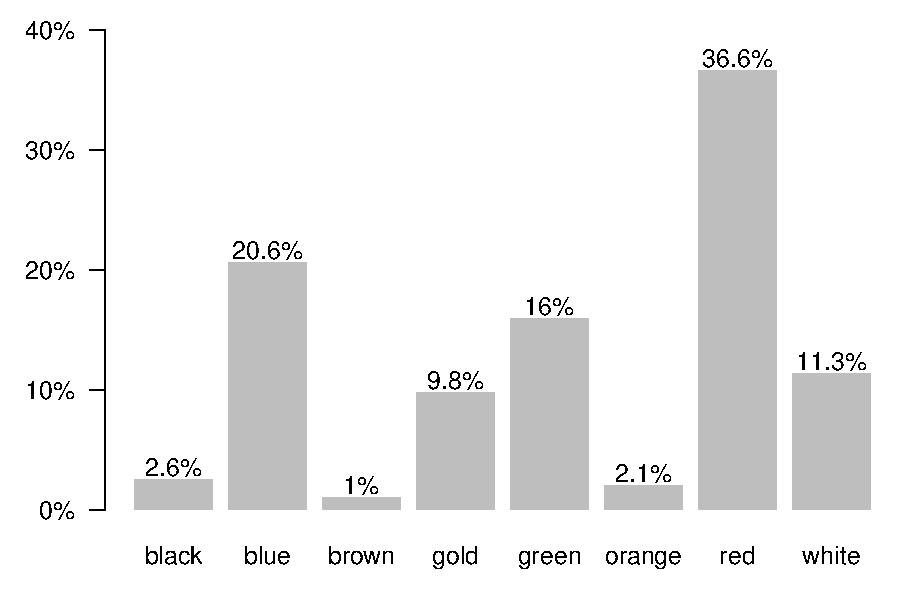
\includegraphics[width=.8\linewidth,height=.6\linewidth]{figure/unnamed-chunk-5-1} 

}



\end{knitrout}

\end{frame}

%------------------------------------------------

\begin{frame}[fragile]
\frametitle{Bar-chart: predominant color in flags}

\begin{knitrout}\footnotesize
\definecolor{shadecolor}{rgb}{0.969, 0.969, 0.969}\color{fgcolor}

{\centering 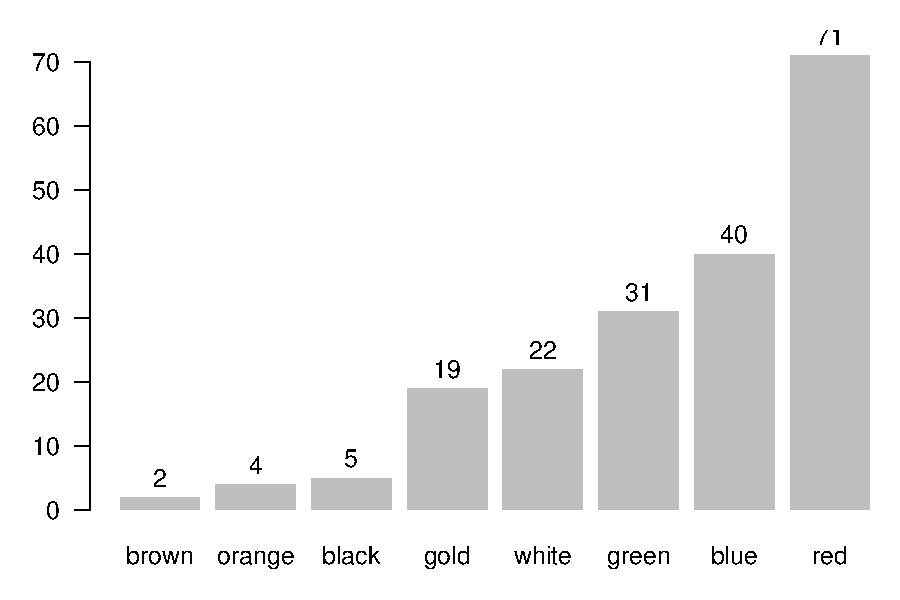
\includegraphics[width=.8\linewidth,height=.6\linewidth]{figure/unnamed-chunk-6-1} 

}



\end{knitrout}

\end{frame}

%------------------------------------------------

\begin{frame}[fragile]
\frametitle{Bar-chart: predominant color in flags}

\begin{knitrout}\footnotesize
\definecolor{shadecolor}{rgb}{0.969, 0.969, 0.969}\color{fgcolor}

{\centering 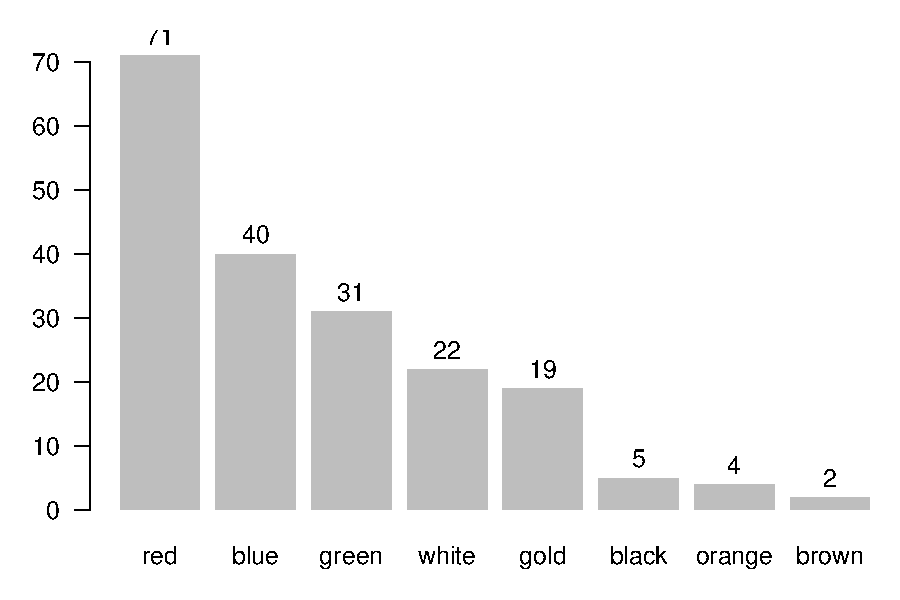
\includegraphics[width=.8\linewidth,height=.6\linewidth]{figure/unnamed-chunk-7-1} 

}



\end{knitrout}

\end{frame}

%------------------------------------------------

\begin{frame}[fragile]
\frametitle{Bar-chart: predominant color in flags}

\begin{knitrout}\footnotesize
\definecolor{shadecolor}{rgb}{0.969, 0.969, 0.969}\color{fgcolor}

{\centering 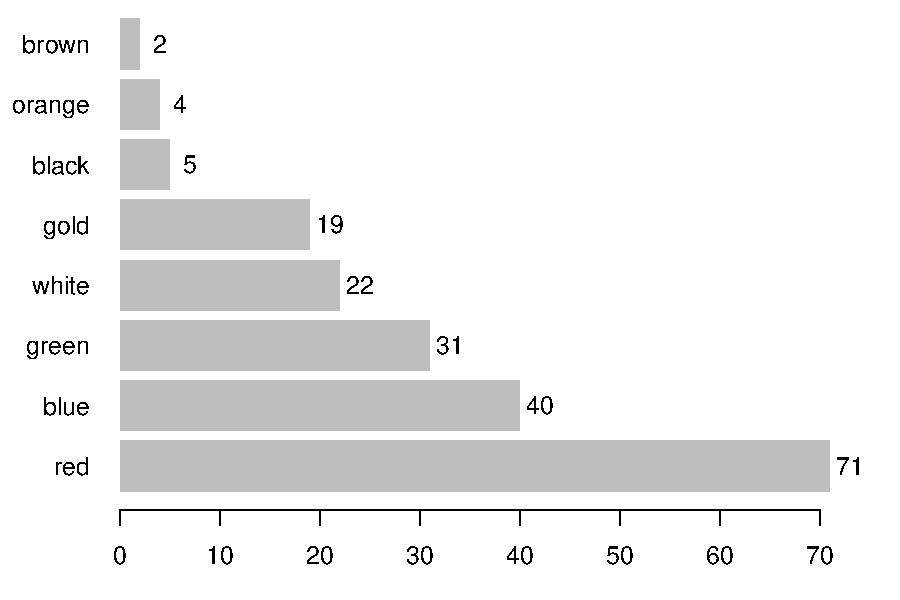
\includegraphics[width=.8\linewidth,height=.6\linewidth]{figure/unnamed-chunk-8-1} 

}



\end{knitrout}

\end{frame}

%------------------------------------------------

\begin{frame}
\begin{center}
\Huge{\hilit{Dot charts}}
\end{center}
\end{frame}

%------------------------------------------------

\begin{frame}
\frametitle{Dot charts}
\bbi
  \item Dot-charts are very similar to bar charts.
  \item Instead of using bars, dot-charts display frequencies with dots.
  \item They are simpler and cleaner than bar charts
  \item They are also less used than bar charts
\ei
\end{frame}

%------------------------------------------------

\begin{frame}[fragile]
\frametitle{Dot-chart: predominant color in flags}

\begin{knitrout}\footnotesize
\definecolor{shadecolor}{rgb}{0.969, 0.969, 0.969}\color{fgcolor}

{\centering 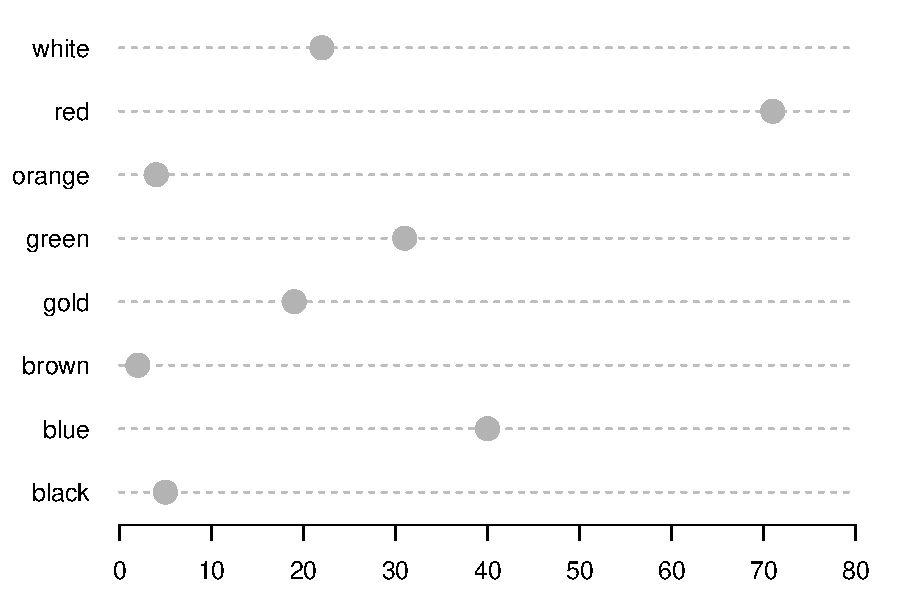
\includegraphics[width=.8\linewidth,height=.6\linewidth]{figure/unnamed-chunk-9-1} 

}



\end{knitrout}

\end{frame}

%------------------------------------------------

\begin{frame}[fragile]
\frametitle{Ranked Dot-charts}

\begin{knitrout}\footnotesize
\definecolor{shadecolor}{rgb}{0.969, 0.969, 0.969}\color{fgcolor}

{\centering 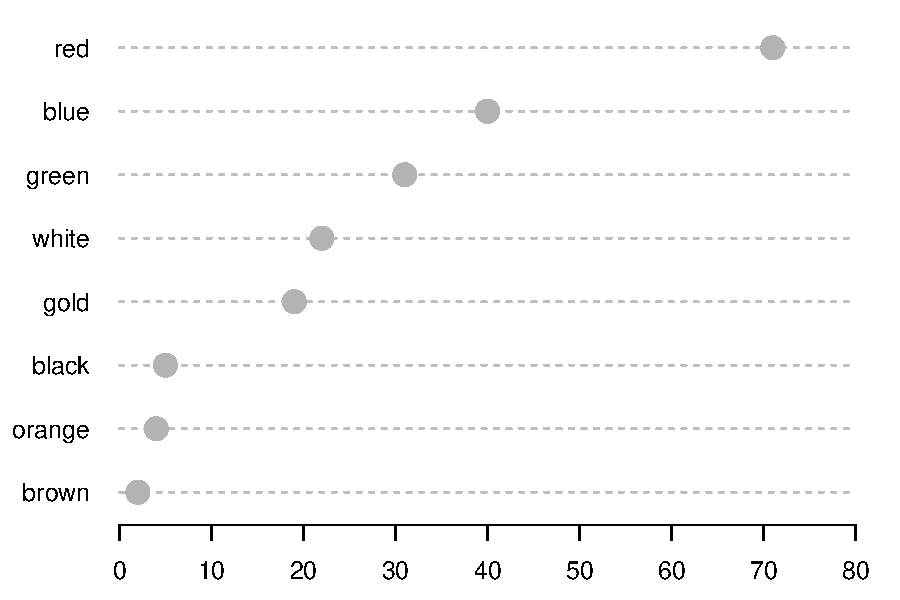
\includegraphics[width=.8\linewidth,height=.6\linewidth]{figure/unnamed-chunk-10-1} 

}



\end{knitrout}

\end{frame}

%------------------------------------------------

\begin{frame}
\frametitle{Ranked dot-chart patterns}
\begin{center}
\ig[width=9cm]{images/dotchart-patterns1.pdf}
\end{center}
\end{frame}

%------------------------------------------------

\begin{frame}
\frametitle{Ranked dot-chart patterns}
\begin{center}
\ig[width=9cm]{images/dotchart-patterns2.pdf}
\end{center}
\end{frame}

%------------------------------------------------

\begin{frame}
\begin{center}
\Huge{\hilit{Pareto charts}}
\end{center}
\end{frame}

%------------------------------------------------

\begin{frame}[fragile]
\frametitle{Bar-chart with Pareto Line}

\begin{knitrout}\footnotesize
\definecolor{shadecolor}{rgb}{0.969, 0.969, 0.969}\color{fgcolor}

{\centering 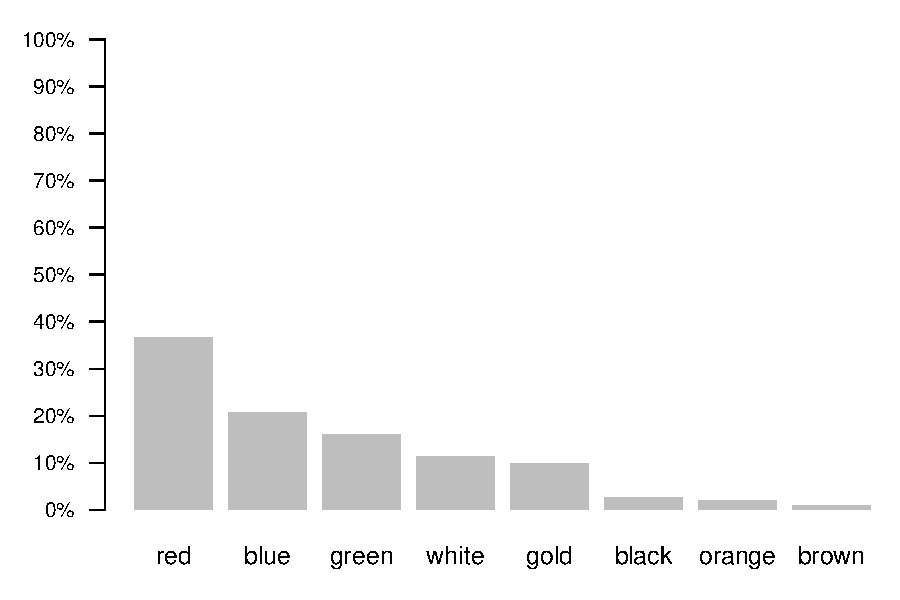
\includegraphics[width=.8\linewidth,height=.6\linewidth]{figure/unnamed-chunk-11-1} 

}



\end{knitrout}

\end{frame}

%------------------------------------------------

\begin{frame}[fragile]
\frametitle{Bar-chart with Pareto Line}

\begin{knitrout}\footnotesize
\definecolor{shadecolor}{rgb}{0.969, 0.969, 0.969}\color{fgcolor}

{\centering 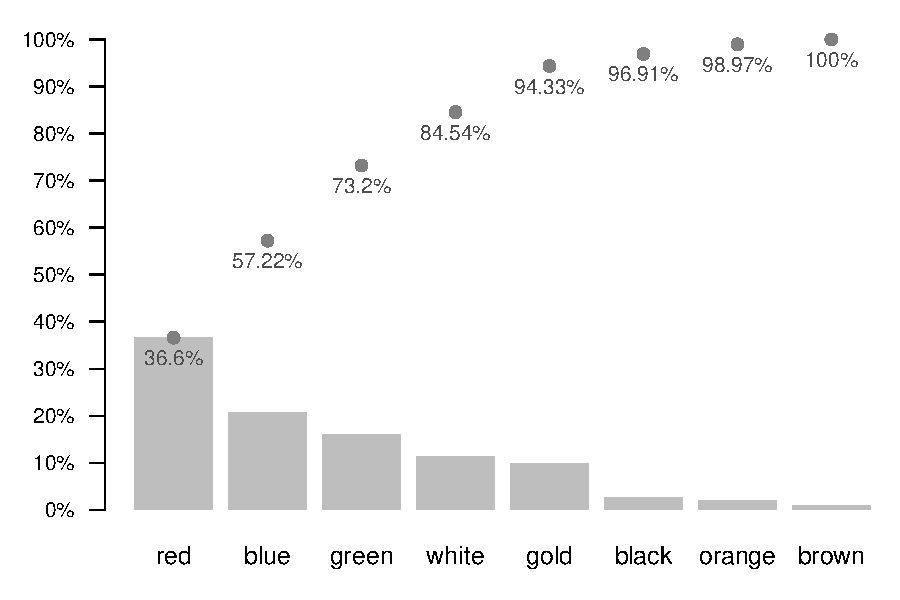
\includegraphics[width=.8\linewidth,height=.6\linewidth]{figure/unnamed-chunk-12-1} 

}



\end{knitrout}

\end{frame}

%------------------------------------------------

\begin{frame}[fragile]
\frametitle{Bar-chart with Pareto Line}

\begin{knitrout}\footnotesize
\definecolor{shadecolor}{rgb}{0.969, 0.969, 0.969}\color{fgcolor}

{\centering 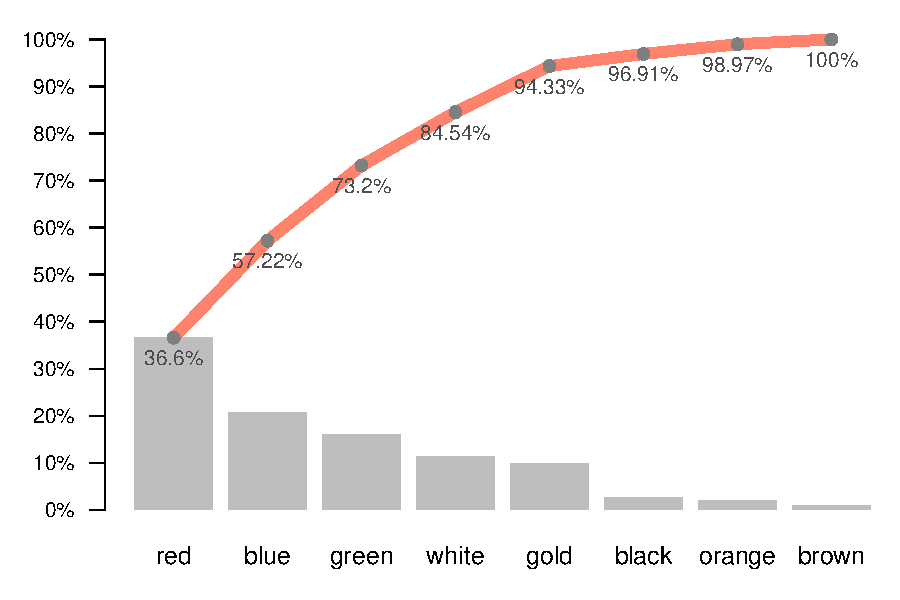
\includegraphics[width=.8\linewidth,height=.6\linewidth]{figure/unnamed-chunk-13-1} 

}



\end{knitrout}

\end{frame}

%------------------------------------------------

\begin{frame}
\frametitle{Pareto charts}
\bbi
  \item Pareto charts contains both bars and a line graph
  \item Individual values are representing in descending order
  \item Cumulative frequencies are represented by the line
  \item The left vertical axis is the frequency of occurrence
\ei
\end{frame}

%------------------------------------------------

\begin{frame}
\begin{center}
\Huge{\hilit{Pie charts}}
\end{center}
\end{frame}

%------------------------------------------------

\begin{frame}[fragile]
\frametitle{Pie Chart}

\begin{knitrout}\footnotesize
\definecolor{shadecolor}{rgb}{0.969, 0.969, 0.969}\color{fgcolor}

{\centering 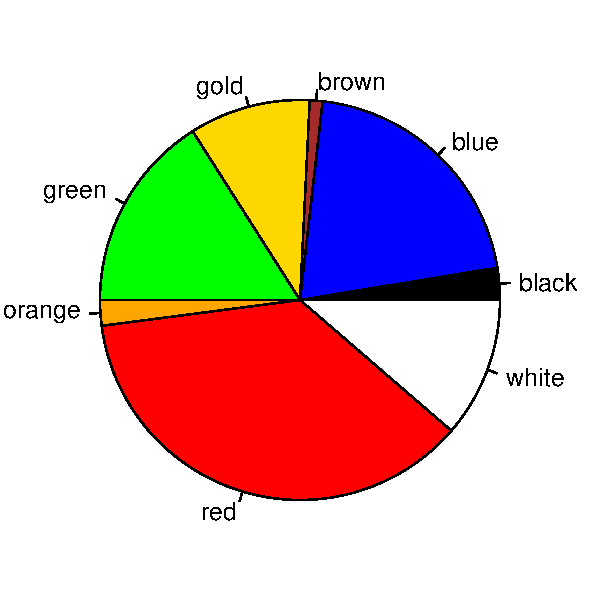
\includegraphics[width=.6\linewidth,height=.6\linewidth]{figure/unnamed-chunk-14-1} 

}



\end{knitrout}

\end{frame}

%------------------------------------------------

\begin{frame}[fragile]
\frametitle{Donut Chart}

\begin{knitrout}\footnotesize
\definecolor{shadecolor}{rgb}{0.969, 0.969, 0.969}\color{fgcolor}

{\centering 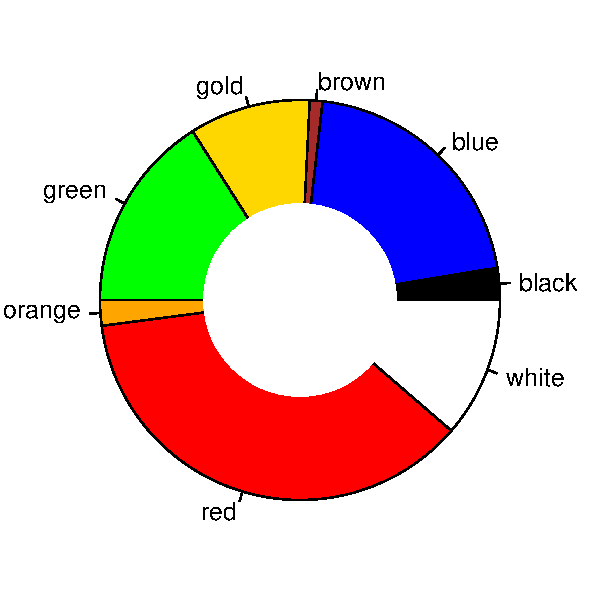
\includegraphics[width=.6\linewidth,height=.6\linewidth]{figure/unnamed-chunk-15-1} 

}



\end{knitrout}

\end{frame}

%------------------------------------------------

\begin{frame}
\frametitle{Pie charts disadvantages}
\bbi
  \item Pie charts force us to compare either 2-D areas formed by each slice or the angles formed
  \item Visual perception handles neitheir of these comparisons easily or accurately
\ei
\end{frame}

%------------------------------------------------

\begin{frame}
\begin{center}
\Huge{\hilit{Univariate Quantitative Charts}}
\end{center}
\end{frame}

%------------------------------------------------

\begin{frame}[fragile]
\frametitle{NFL Ticket prices (2013)}
\begin{knitrout}\footnotesize
\definecolor{shadecolor}{rgb}{0.969, 0.969, 0.969}\color{fgcolor}\begin{kframe}
\begin{verbatim}
##        teams  tickets       teams  tickets
## 1    cowboys   110.20     falcons    83.71
## 2   patriots   117.84     vikings    78.69
## 3     giants   111.69        rams    74.49
## 4      bears   103.60    seahawks    71.21
## 5       jets   110.28   cardinals    79.56
## 6   redskins    94.80    dolphins    71.14
## 7     ravens   100.19     raiders    64.80
## 8     eagles    93.01      titans    65.28
## 9     texans    88.98       lions    67.60
## 10  chargers    84.55     bengals    68.96
## 11  steelers    81.13     jaguars    68.44
## 12   packers    82.61      chiefs    64.92
## 13     49ers    83.54  buccaneers    63.59
## 14    saints    74.99       bills    57.75
## 15   broncos    84.27    panthers    66.84
## 16     colts    86.32      browns    54.20
\end{verbatim}
\end{kframe}
\end{knitrout}
\end{frame}

%------------------------------------------------

\begin{frame}
\frametitle{Bar charts for quantitative variables}
\bbi
  \item We can use bar charts with quantitative variables
  \item In this case we need to first categorize the variable, and then get a frequency table
\ei
\end{frame}

%------------------------------------------------

\begin{frame}
\frametitle{Frequency Table of Ticket Prices}

{\large
\begin{center}
 \begin{tabular}{c c c}
  \hline
  Category & Absolute & Relative \\
  Name & Frequency & Frequency \\
  \hline
  Below \$70 & 10 & 0.3125 \\
  \$70 - \$99.99 & 16 & 0.5000 \\
  \$100 or above & 6 & 0.1875 \\
  \hline
  Total & 32 & 1.00 \\
 \end{tabular}
\end{center}
}

\end{frame}

%------------------------------------------------

\begin{frame}[fragile]
\frametitle{NFL Ticket prices (2013)}
\begin{knitrout}\footnotesize
\definecolor{shadecolor}{rgb}{0.969, 0.969, 0.969}\color{fgcolor}

{\centering 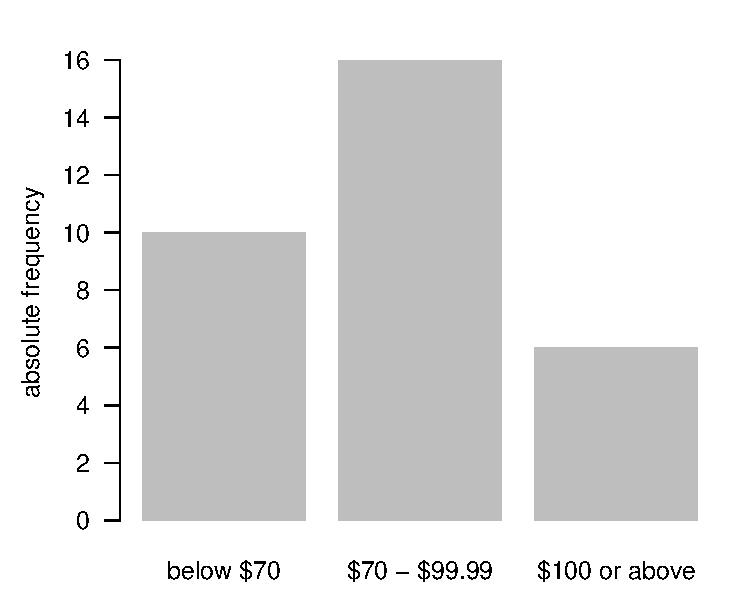
\includegraphics[width=.7\linewidth,height=.6\linewidth]{figure/unnamed-chunk-17-1} 

}



\end{knitrout}

\end{frame}

%------------------------------------------------

\begin{frame}
\begin{center}
\Huge{\hilit{Histograms}}
\end{center}
\end{frame}

%------------------------------------------------

\begin{frame}
\frametitle{Histograms}
Histograms provide a way of viewing the general distribution of values in a quantitative variable
\end{frame}

%------------------------------------------------

\begin{frame}[fragile]
\frametitle{NFL Ticket prices (2013)}
\begin{knitrout}\footnotesize
\definecolor{shadecolor}{rgb}{0.969, 0.969, 0.969}\color{fgcolor}

{\centering 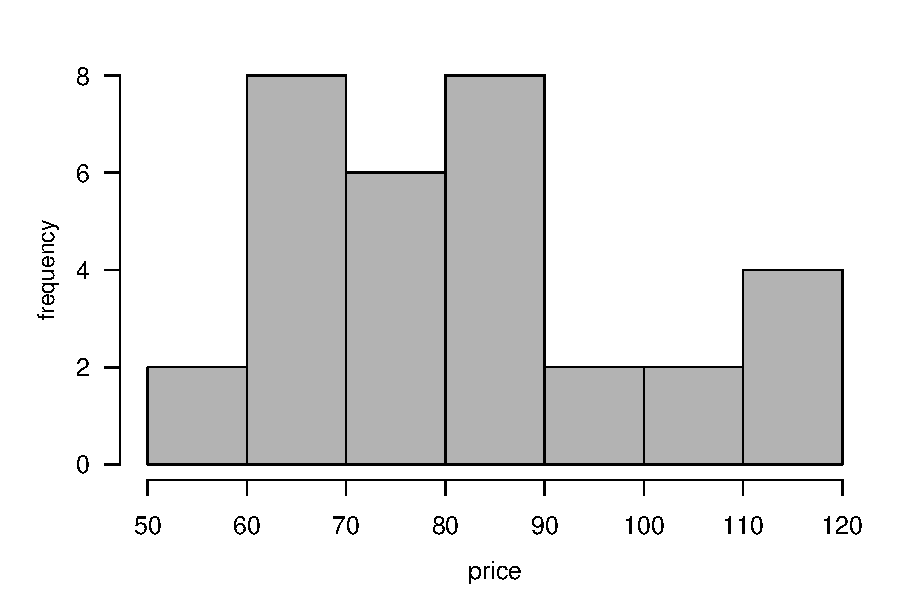
\includegraphics[width=.8\linewidth,height=.6\linewidth]{figure/unnamed-chunk-18-1} 

}



\end{knitrout}

\end{frame}

%------------------------------------------------

\begin{frame}
\frametitle{Building a Histogram}

\begin{enumerate}
  \item \textbf{Partition of values}: The range of the data values is partitioned into a number of non-overlapping ``cells'' or bins.
  \item \textbf{Counting frequencies}: The number of data values falling into each cell is counted (either absolute or relative freqs)
  \item \textbf{Drawing Bars}: The observations falling into a cell are represented as a ``bar'' drawn over the cell
\end{enumerate}

\end{frame}

%------------------------------------------------

\begin{frame}
\frametitle{About Histograms}

\bi
  \item The bins represent ranges of values
  \item The bins (intervals) must be adjacent, and usually of equal size
  \item The bars are adjacent (not discontinuous)
  \item The areas of the bars are meaningful
  \item Height of bars equal to the frequency
  \item Width equal to the bin size
  \item The area of a bar gives the proportion of data values which fall in the bin
\ei

\end{frame}

%------------------------------------------------

\begin{frame}[fragile]
\frametitle{Histogram with 4 bins}
\begin{knitrout}\footnotesize
\definecolor{shadecolor}{rgb}{0.969, 0.969, 0.969}\color{fgcolor}

{\centering 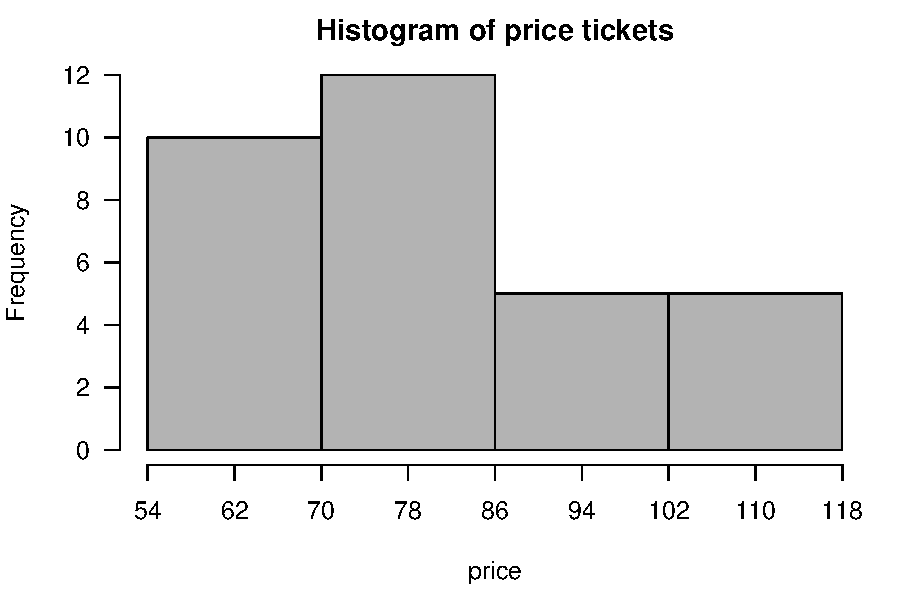
\includegraphics[width=.8\linewidth,height=.6\linewidth]{figure/unnamed-chunk-19-1} 

}



\end{knitrout}

\end{frame}

%------------------------------------------------

\begin{frame}[fragile]
\frametitle{Histograms with different bins}
\begin{knitrout}\footnotesize
\definecolor{shadecolor}{rgb}{0.969, 0.969, 0.969}\color{fgcolor}

{\centering 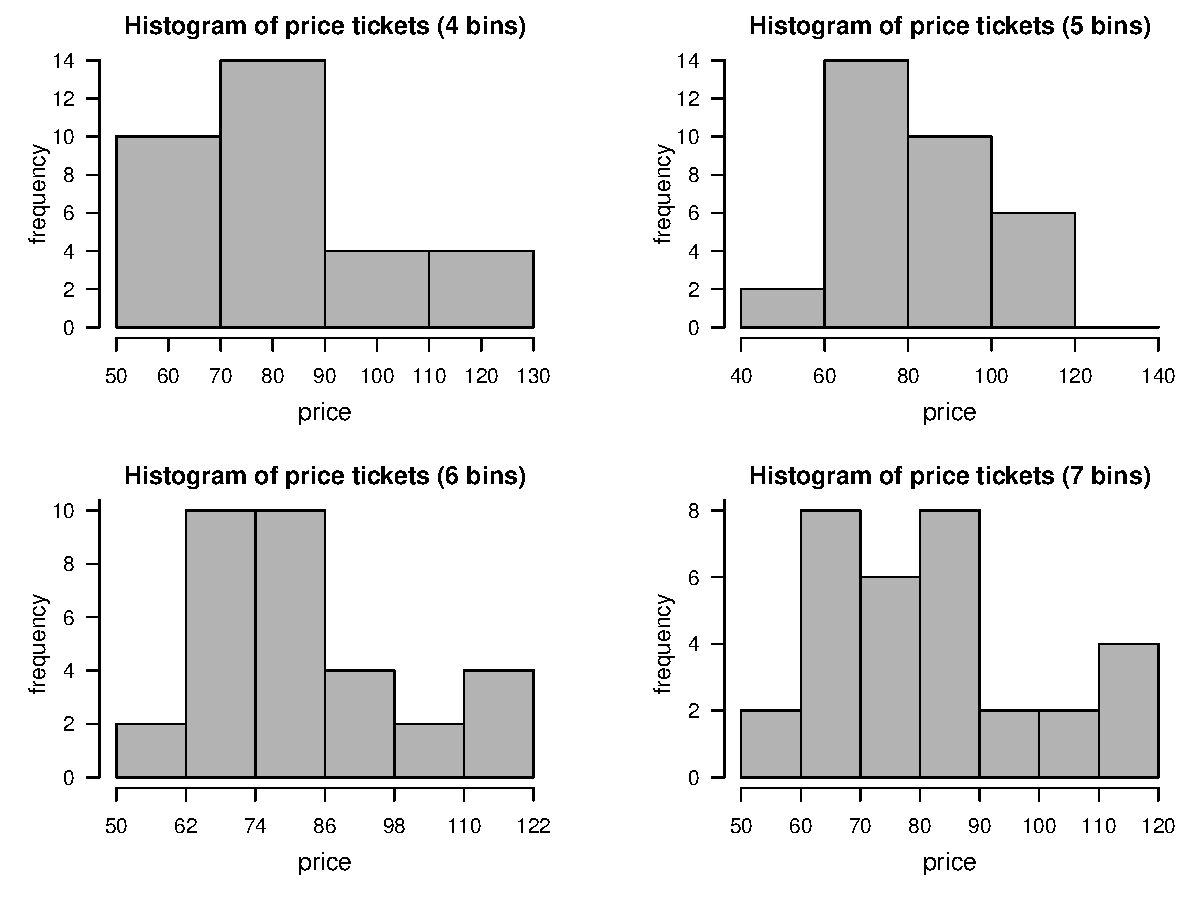
\includegraphics[width=.9\linewidth,height=.7\linewidth]{figure/unnamed-chunk-20-1} 

}



\end{knitrout}

\end{frame}

%------------------------------------------------

\begin{frame}[fragile]
\frametitle{Avoid too few and too many bins}
\begin{knitrout}\footnotesize
\definecolor{shadecolor}{rgb}{0.969, 0.969, 0.969}\color{fgcolor}

{\centering 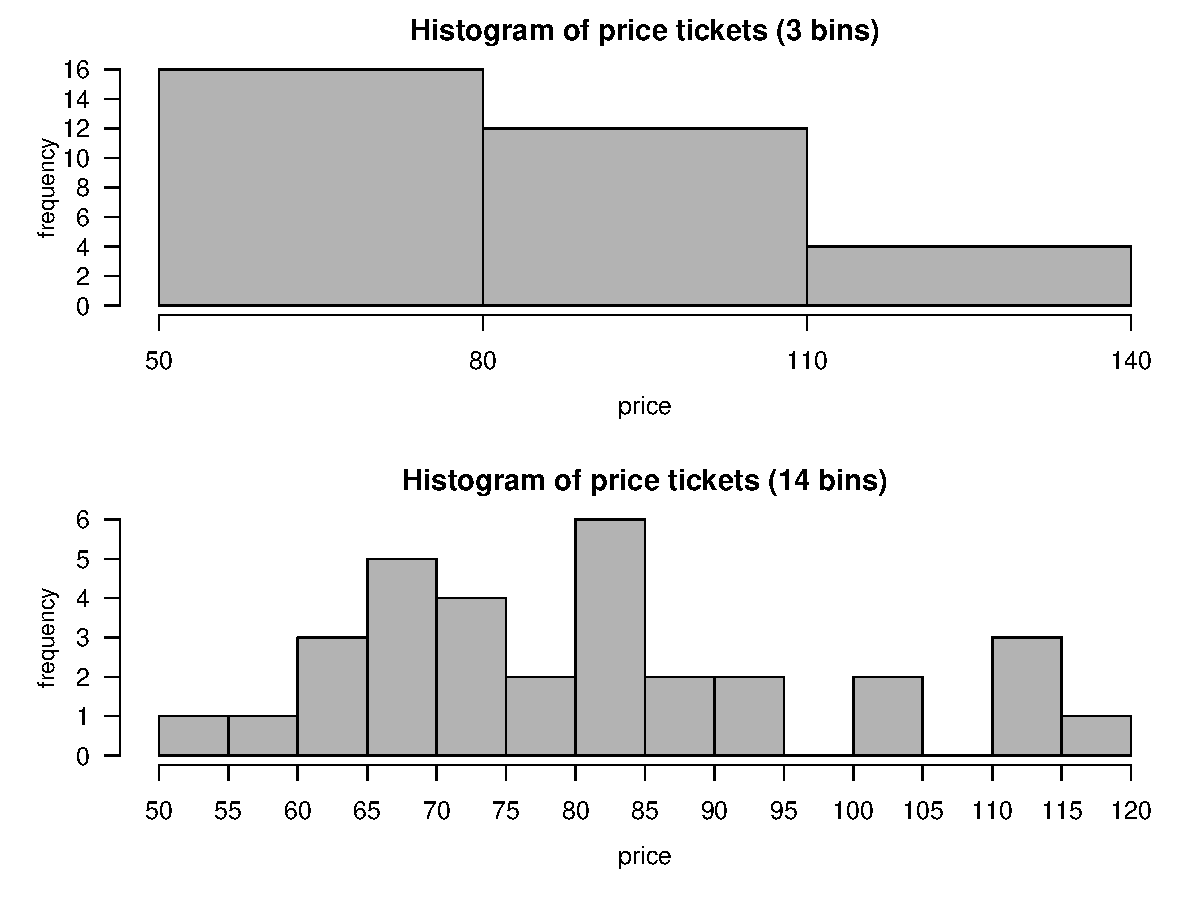
\includegraphics[width=.9\linewidth,height=.7\linewidth]{figure/unnamed-chunk-21-1} 

}



\end{knitrout}

\end{frame}

%------------------------------------------------

\begin{frame}
\frametitle{About Histograms}

\bi
  \item The shape of a histogram depends on the chosen bins
  \item This suggests that there is a fundamental instability at the heart of its construction
  \item The bars are adjacent (not discontinuous)
  \item The areas of the bars are meaningful
\ei

\end{frame}

%------------------------------------------------

\begin{frame}
\frametitle{Histogram patterns}
\begin{center}
\ig[width=9cm]{images/histogram-skew.pdf}
\end{center}
\end{frame}

%------------------------------------------------

\begin{frame}
\frametitle{Histogram patterns}
\begin{center}
\ig[width=9cm]{images/histogram-profiles1.pdf}
\end{center}
\end{frame}

%------------------------------------------------

\begin{frame}
\frametitle{Histogram patterns}
\begin{center}
\ig[width=9cm]{images/histogram-profiles2.pdf}
\end{center}
\end{frame}

%------------------------------------------------

\begin{frame}
\frametitle{Histogram patterns}
\begin{center}
\ig[width=9cm]{images/histogram-shapes.pdf}
\end{center}
\end{frame}

%------------------------------------------------

\begin{frame}
\begin{center}
\Huge{\hilit{Box plots}}
\end{center}
\end{frame}

%------------------------------------------------

\begin{frame}
\frametitle{Building a Histogram}

\begin{enumerate}
  \item \textbf{Box-and-whisker plots}, most commonly known as ``box plots''
  \item created by John Tukey
  \item simple and effective way to display the distribution of values
  \item relies on the so-called \textbf{5-summary indicators}
\end{enumerate}

\end{frame}

%------------------------------------------------

\begin{frame}
\frametitle{Box plots based on 5-number summary}

\bb{5 summary indicators}
\pause
\begin{enumerate}
  \item minimum
  \item 25th percentile (1st quartile)
  \item 50th percentile (2nd quartile, or median)
  \item 75th percentile (3rd quartile)
  \item maximum
\end{enumerate}
\eb

\end{frame}

%------------------------------------------------

\begin{frame}
\frametitle{Box plot basics}
\begin{center}
\ig[height=6cm]{images/boxplot1.pdf}
\end{center}
\end{frame}

%------------------------------------------------

\begin{frame}
\frametitle{Box plot basics}
\begin{center}
\ig[height=6cm]{images/boxplot2.pdf}
\end{center}
\end{frame}

%------------------------------------------------

\begin{frame}[fragile]
\frametitle{NFL Ticket Prices}
\begin{knitrout}\footnotesize
\definecolor{shadecolor}{rgb}{0.969, 0.969, 0.969}\color{fgcolor}

{\centering 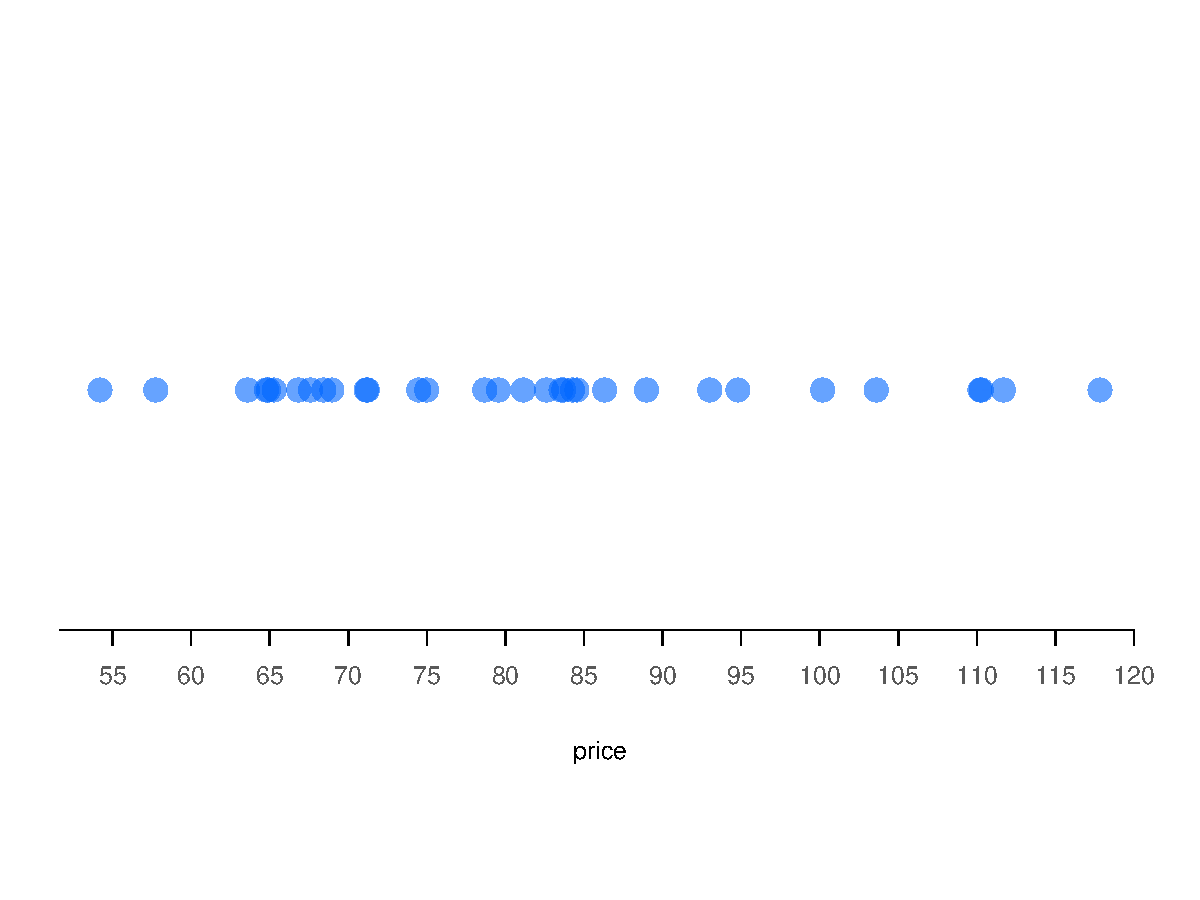
\includegraphics[width=.9\linewidth,height=.7\linewidth]{figure/unnamed-chunk-22-1} 

}



\end{knitrout}

\end{frame}

%------------------------------------------------

\begin{frame}[fragile]
\frametitle{5 number summary}
\begin{knitrout}\footnotesize
\definecolor{shadecolor}{rgb}{0.969, 0.969, 0.969}\color{fgcolor}

{\centering 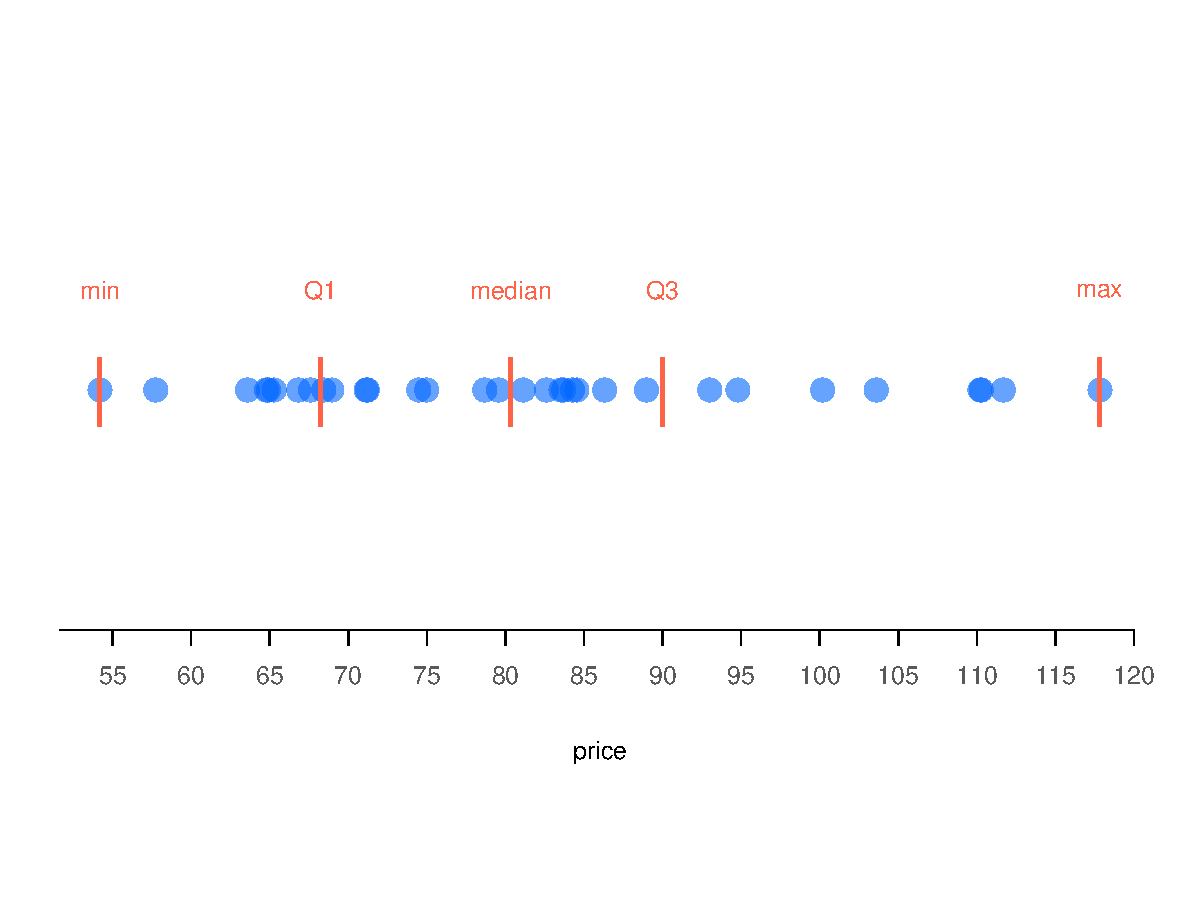
\includegraphics[width=.9\linewidth,height=.7\linewidth]{figure/unnamed-chunk-23-1} 

}



\end{knitrout}

\end{frame}

%------------------------------------------------

\begin{frame}[fragile]
\frametitle{Box plot}
\begin{knitrout}\footnotesize
\definecolor{shadecolor}{rgb}{0.969, 0.969, 0.969}\color{fgcolor}

{\centering 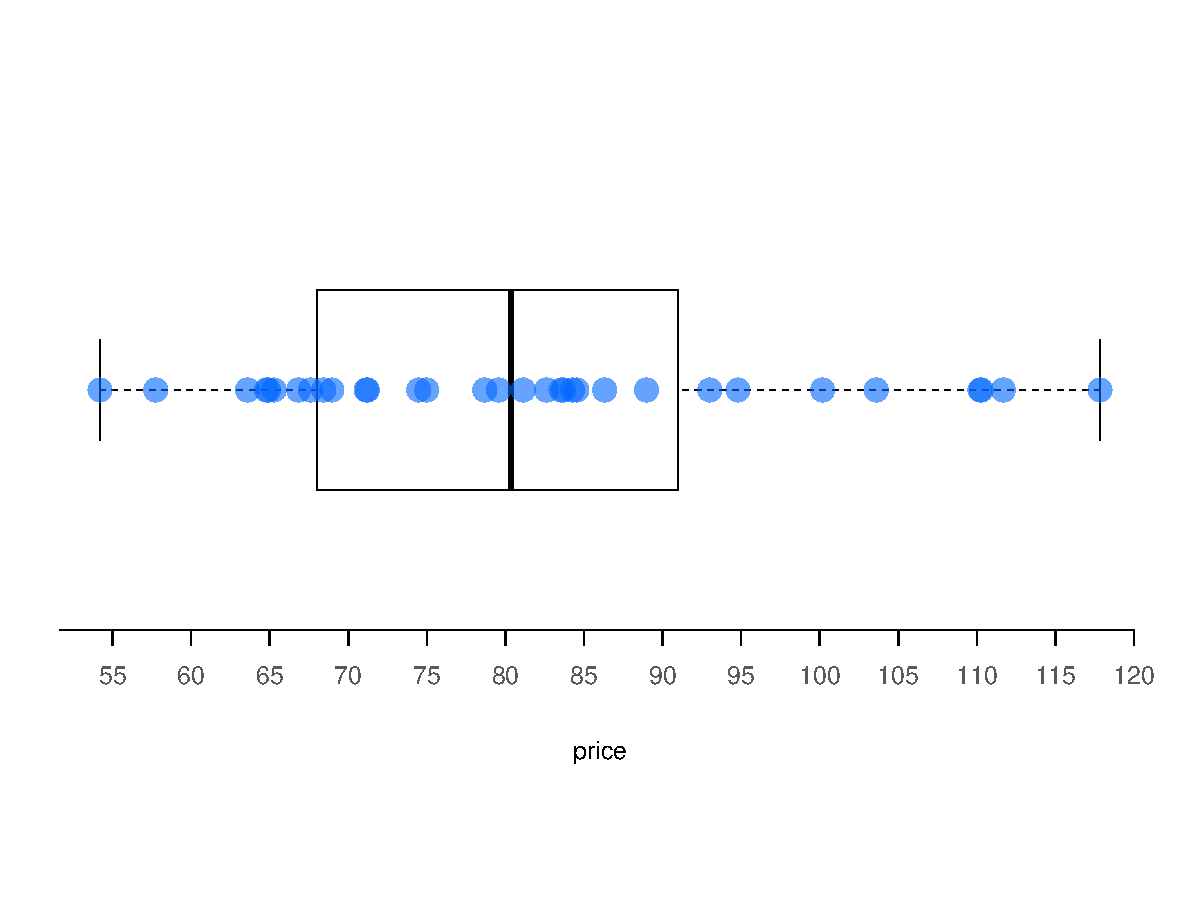
\includegraphics[width=.9\linewidth,height=.7\linewidth]{figure/unnamed-chunk-24-1} 

}



\end{knitrout}

\end{frame}

%------------------------------------------------

\begin{frame}[fragile]
\frametitle{Box plot}
\begin{knitrout}\footnotesize
\definecolor{shadecolor}{rgb}{0.969, 0.969, 0.969}\color{fgcolor}

{\centering 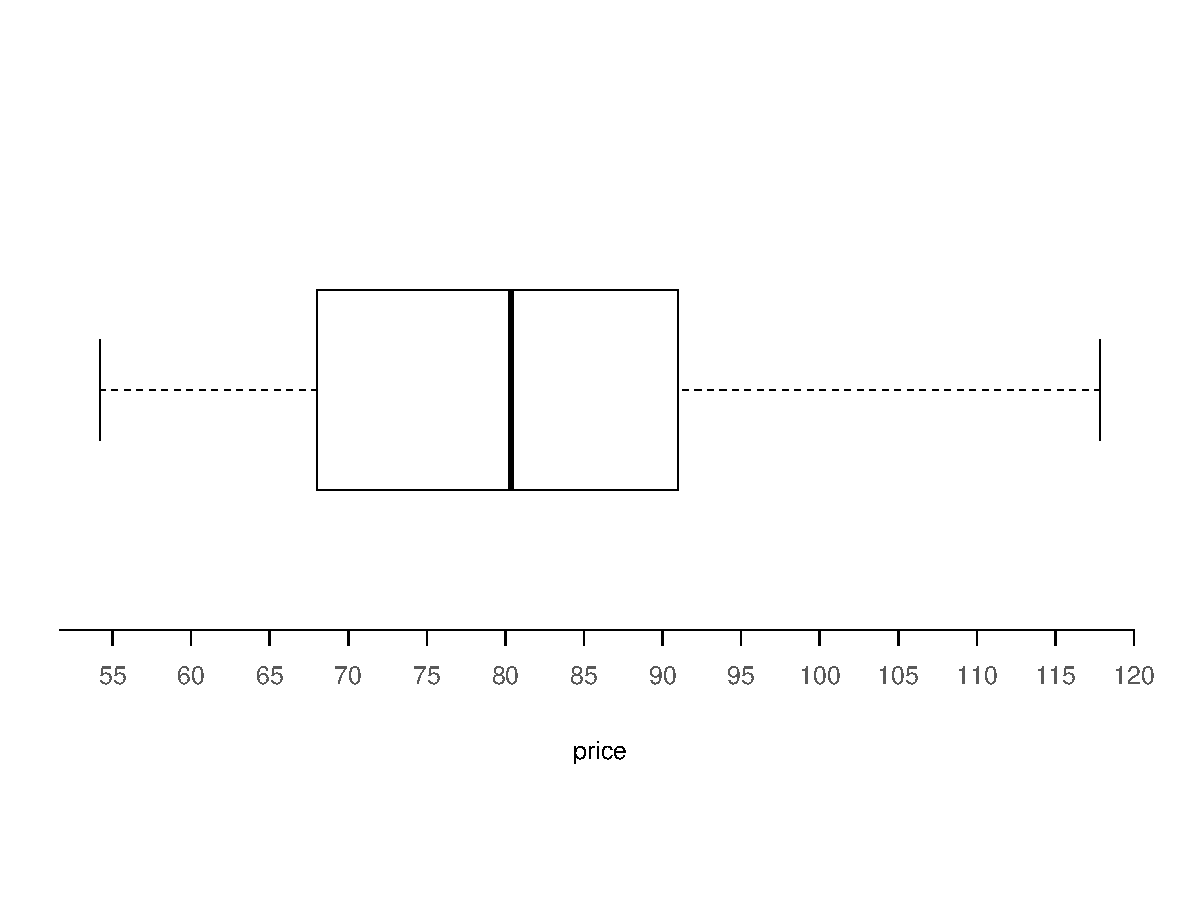
\includegraphics[width=.9\linewidth,height=.7\linewidth]{figure/unnamed-chunk-25-1} 

}



\end{knitrout}

\end{frame}

%------------------------------------------------

\begin{frame}
\frametitle{Box plot and outliers}

\bb{The 1.5 x IQR rule for outliers}
Call an observation a suspected outlier if it falls more than {\hilit 1.5 x IQR} above the third quartile or below the first quartile
\eb
\end{frame}

%------------------------------------------------

\begin{frame}
\frametitle{Modified Box plot}
\begin{center}
\ig[width=9cm]{images/boxplot-modified.pdf}
\end{center}
\end{frame}

%------------------------------------------------

\begin{frame}
\begin{center}
\Huge{\hilit{Density Curves}}
\end{center}
\end{frame}

%------------------------------------------------

\begin{frame}[fragile]
\frametitle{Density Curve}
\begin{knitrout}\footnotesize
\definecolor{shadecolor}{rgb}{0.969, 0.969, 0.969}\color{fgcolor}

{\centering 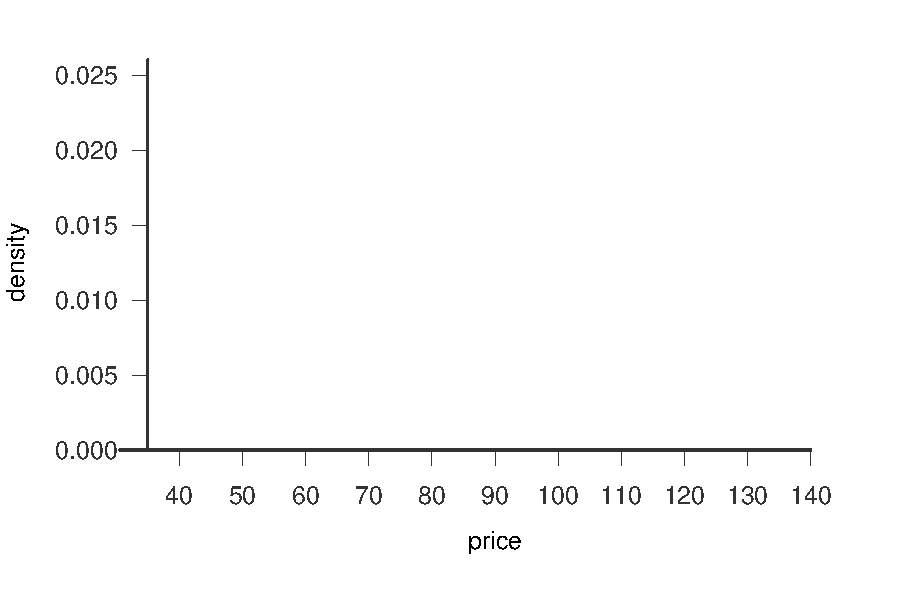
\includegraphics[width=.8\linewidth,height=.6\linewidth]{figure/unnamed-chunk-26-1} 

}



\end{knitrout}

\end{frame}

%------------------------------------------------

\begin{frame}
\frametitle{Density Curve}

\bb{A Density Curve}
\bi
  \item Describes the distribution of values by a smooth curve
  \item Is always on or above the horizontal axis
  \item Has area equal to 1 underneath it
  \item Is an idealized distribution
\ei
\eb

\end{frame}

%------------------------------------------------

\begin{frame}
\frametitle{Density Curve}

\bb{About Density Curve}
\bi
  \item The \textbf{mode} is the peak point of the curve (could be more than one or none)
  \item The \textbf{median} is the equal-areas point
  \item The \textbf{mean} is the balance point
  \item The median and the mean are always equal on a symmetric density curve
\ei
\eb

\end{frame}

%------------------------------------------------

\begin{frame}
\begin{center}
\Huge{\hilit{Ogives}}
\end{center}
\end{frame}

%------------------------------------------------

\begin{frame}
\frametitle{Ogives}

\bb{About Ogives}
\bbi
  \item Ogives help us examine the cumulative distribution of values in a quantitative variable
  \item An ogive tells us how many data are less than the indicated value on the horizontal axis
  \item An ogive shows how slowly or rapidly the data values accumulate over the range of the data
\ei
\eb

\end{frame}

%------------------------------------------------

\begin{frame}
\frametitle{Frequency Table NFL Price Tickets}

\begin{center}
 \begin{tabular}{c c c c c}
  \hline
  Bin & Interval & Mid-point & Frequency & Cum Freq \\
  \hline
  1 & [50-60) & 55 & 2 & 2 \\
  2 & [60-70) & 65 & 8 & 10 \\
  3 & [70-80) & 75 & 6 & 16 \\
  4 & [80-90) & 85 & 8 & 24 \\
  5 & [90-100) & 95 & 2 & 26 \\
  6 & [100-110) & 105 & 2 & 28 \\
  7 & [110-120) & 115 & 4 & 32 \\
 \end{tabular}
\end{center}

\end{frame}

%------------------------------------------------

\begin{frame}[fragile]
\frametitle{Ogive}
\begin{knitrout}\footnotesize
\definecolor{shadecolor}{rgb}{0.969, 0.969, 0.969}\color{fgcolor}

{\centering 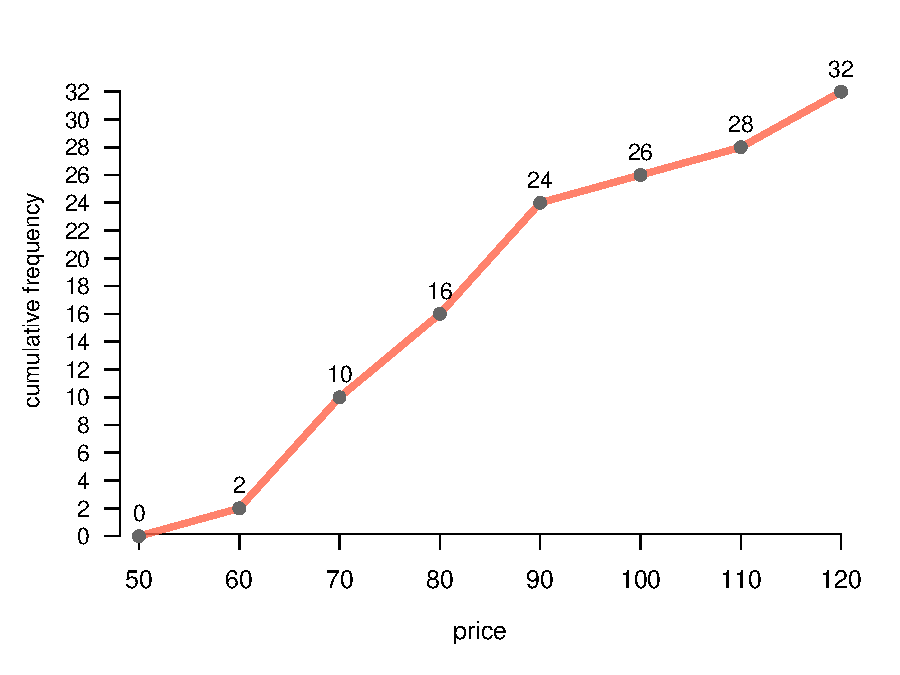
\includegraphics[width=.9\linewidth,height=.65\linewidth]{figure/unnamed-chunk-27-1} 

}



\end{knitrout}

\end{frame}

%------------------------------------------------

\begin{frame}
\frametitle{Ogives}

\bb{Building an Ogive}
\bbi
  \item Make a frequency table showing bin intervals and cumulative frequencies.
  \item An ogive begins on the horizontal axis at the lower boundary of the first bin.
  \item For each bin, make a dot over the upper interval limit at the height of the cumulative frequency.
  \item Connect the dots with line segments.
\ei
\eb

\end{frame}

%------------------------------------------------

\begin{frame}
\begin{center}
\Huge{\hilit{Distributions and Ogives}}
\end{center}
\end{frame}

%------------------------------------------------

\begin{frame}[fragile]
\frametitle{Three histograms}
\begin{knitrout}\footnotesize
\definecolor{shadecolor}{rgb}{0.969, 0.969, 0.969}\color{fgcolor}

{\centering 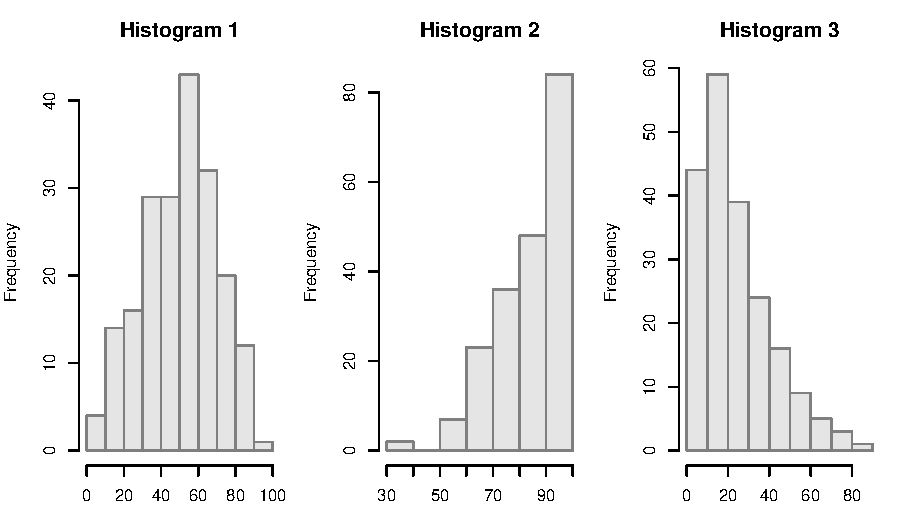
\includegraphics[width=.9\linewidth,height=.5\linewidth]{figure/unnamed-chunk-28-1} 

}



\end{knitrout}

\end{frame}

%------------------------------------------------

\begin{frame}[fragile]
\frametitle{Symmetric Distribution}


\begin{knitrout}\footnotesize
\definecolor{shadecolor}{rgb}{0.969, 0.969, 0.969}\color{fgcolor}

{\centering 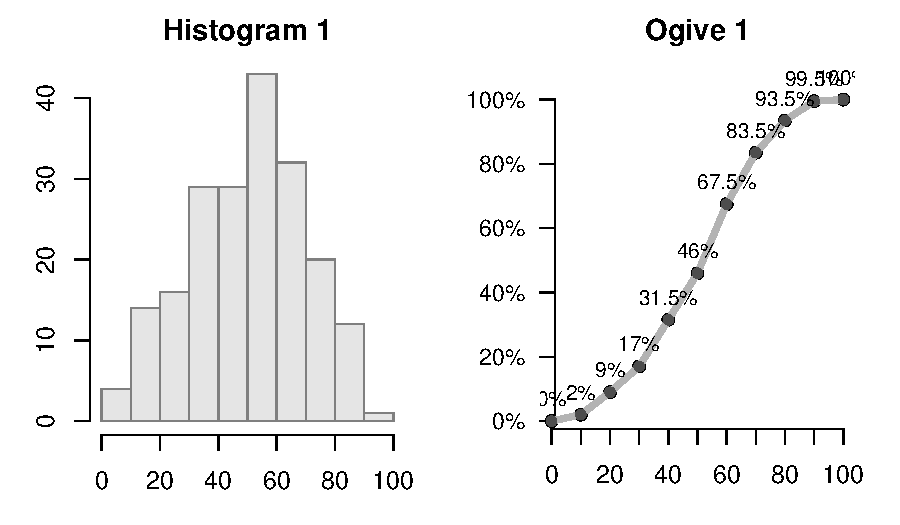
\includegraphics[width=.9\linewidth,height=.5\linewidth]{figure/unnamed-chunk-30-1} 

}



\end{knitrout}

\end{frame}

%------------------------------------------------

\begin{frame}[fragile]
\frametitle{Skewed to the left Distribution}

\begin{knitrout}\footnotesize
\definecolor{shadecolor}{rgb}{0.969, 0.969, 0.969}\color{fgcolor}

{\centering 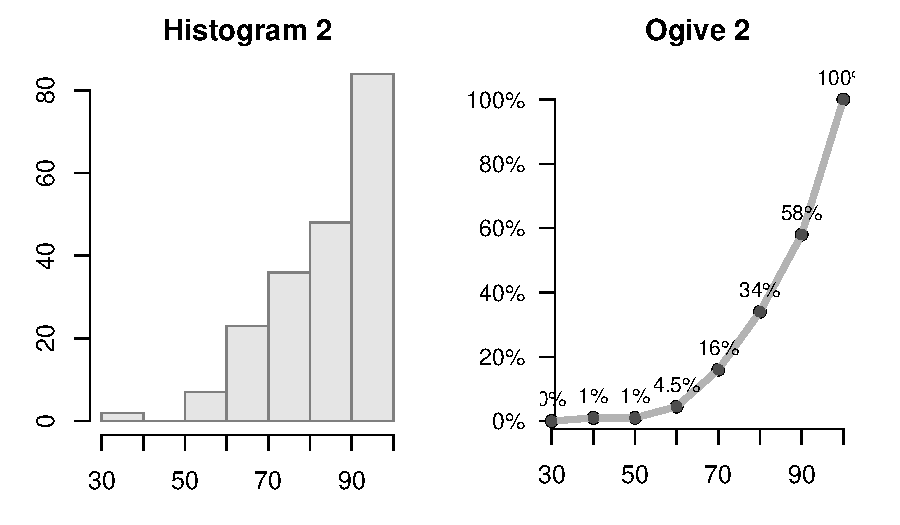
\includegraphics[width=.9\linewidth,height=.5\linewidth]{figure/unnamed-chunk-31-1} 

}



\end{knitrout}

\end{frame}

%------------------------------------------------

\begin{frame}[fragile]
\frametitle{Skewed to the right Distribution}

\begin{knitrout}\footnotesize
\definecolor{shadecolor}{rgb}{0.969, 0.969, 0.969}\color{fgcolor}

{\centering 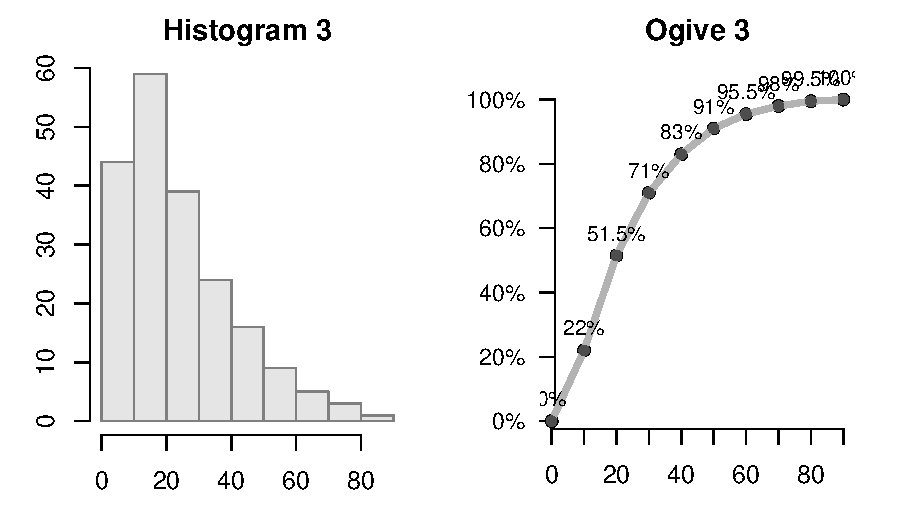
\includegraphics[width=.9\linewidth,height=.5\linewidth]{figure/unnamed-chunk-32-1} 

}



\end{knitrout}

\end{frame}

%------------------------------------------------

\end{document}
